\pdfminorversion=4
\documentclass[letterpaper, 10 pt, conference]{ieeeconf}
% \documentclass[a4paper, 10 pt, conference]{ieeeconf}

\usepackage{times}
\usepackage{graphicx}
\usepackage{wrapfig}
\usepackage{xfrac}

\usepackage{multicol}
\usepackage{amsmath}
\usepackage{siunitx}
\sisetup{range-phrase=--,range-units=single}

\usepackage{circuitikz}
\usetikzlibrary{patterns,hobby,decorations.pathmorphing}

\usepackage{multirow}

\usepackage{makecell}
\renewcommand\theadfont{\bfseries}

\usepackage{booktabs}

\usepackage[hidelinks]{hyperref}
\usepackage{cleveref}
\Crefformat{figure}{#2Fig.~#1#3}
\Crefmultiformat{figure}{Figs.~#2#1#3}{ and~#2#1#3}{, #2#1#3}{ and~#2#1#3}
\crefformat{footnote}{#2\footnotemark[#1]#3}

\IEEEoverridecommandlockouts

\overrideIEEEmargins

\title{\LARGE \bf
Sim2Real for Soft Robotic Fish via Differentiable Simulation
}


\author{John Z. Zhang$^{1,2}$, Yu Zhang$^{1}$, Pingchuan Ma$^{3}$,  Elvis Nava$^{1,4}$, Tao Du$^{3}$, Philip Arm$^{1}$, \\ Wojciech Matusik$^{3}$, Robert K. Katzschmann$^{1,4}$% <-this % stops a space
\thanks{*We are grateful for funding received by the ETH AI Center, and the Defense Advanced Research Projects Agency.}%
\thanks{$^{1}$Soft Robotics Lab, ETH Zurich, Switzerland}%
\thanks{$^{2}$Mechanical Engineering, MIT, USA}%
\thanks{$^{3}$Computer Science and AI Lab, MIT, USA}%
\thanks{$^{4}$ETH AI Center, ETH Zurich, Switzerland}
\thanks{Corresponding author: Robert K. Katzschmann, {\tt\footnotesize 
% \href{mailto:johnz@mit.edu}{johnz@mit.edu}, 
% \href{mailto:zhangyu@ethz.ch}{zhangyu@ethz.ch}, 
% \href{mailto:pcma@mit.edu}{pcma@mit.edu}, 
% \href{mailto:enava@ethz.ch}{enava}@ethz.ch,
% \href{mailto:taodu@csail.mit.edu}{taodu}@csail.mit.edu,
% \href{mailto:parm@ethz.ch}{parm}@ethz.ch,
% \href{mailto:wojciech@csail.mit.edu}{wojciech}@csail.mit.edu, 
\href{mailto:rkk@ethz.ch}{rkk@ethz.ch}}}% <-this % stops a space
}


\begin{document}

\maketitle
\thispagestyle{empty}
\pagestyle{empty}

\begin{abstract}
Accurate simulation of soft mechanisms under dynamic actuation is critical for the design of soft robots.
We address this gap with our differentiable simulation tool by learning the material parameters of our soft robotic fish.
On the example of a soft robotic fish, we demonstrate an experimentally-verified, fast optimization pipeline for learning the material parameters from quasi-static data via differentiable simulation and apply it to the prediction of dynamic performance.
Our method identifies physically plausible Young’s moduli for various soft silicone elastomers and stiff acetal copolymers used in creation of our three different robotic fish tail designs. We show that our method is compatible with varying internal geometry of the actuators, such as the number of hollow cavities.
Our framework allows high fidelity prediction of dynamic behavior for composite bi-morph bending structures in real hardware to millimeter-accuracy and within $3\%$ error normalized to actuator length.
We provide a differentiable and robust estimate of the thrust force using a neural network thrust predictor; this estimate allows for accurate modeling of our experimental setup measuring bollard pull. 
This work presents a prototypical hardware and simulation problem solved using our differentiable framework; the framework can be applied to higher dimensional parameter inference, learning control policies, and computational design due to its differentiable character.
\end{abstract}


version https://git-lfs.github.com/spec/v1
oid sha256:f7f279fa0f93cb2842457a52f2e0361e29261eb78732a2e3ff4c6aebddfefb19
size 6684

version https://git-lfs.github.com/spec/v1
oid sha256:cb323d9fad3db6daf5d284e3e48c0f8f296e1bed741ca4d7f3258f66a71e2940
size 7395

\section{System Overview}
\label{system_overview}

Our pipeline (\Cref{fig:overview}) learns the material parameters of a soft robotic fish (see \Cref{fig:pneumatic_fish_tail}) using differentiable simulation and measurements from quasistatic experiments. Thrust force is simulated using a data-driven neural network predictor. We demonstrate that sim2real matching is good within $3\%$ positional error normalized to actuator length for our soft robotic fish prototypes even under significant bending.

\begin{figure}[tb]
    \centering
    \includegraphics[width=0.48\textwidth]{figures/overview.png}
    \caption{Flow diagram of our differentiable simulation and learning pipeline. To learn the material parameters, we compute the loss as the Euclidean distance between the measured marker positions $\mathbf{x}_\textrm{m}$ and the simulated position data $\mathbf{x}_t$ and then minimize this loss using gradient-search enabled by our differentiable FEM simulation. The marker positions are 2D in-plane measurements primarily due to lateral displacement during flapping. Our neural network thrust predictor takes as input the positions and pressure at a previous time step and outputs the thrust force for the next time step.}
    \label{fig:overview}
\end{figure}

In \Cref{simulation}, forward simulation is accomplished using implicit Euler time stepping and FEM spatial discretization. We leverage projective dynamics for a substantial speed up in computation\,\cite{du2021diffpd}.
We describe our bollard-pull style experimental setup in \Cref{experimental_setup}.
In \Cref{system identification}, the material properties of the body and spine are specified by two different corotated materials stitched together at the boundary.
We verify the results (\Cref{fig:system_id}) of our system identification by comparing simulations to measurements from a gamut of dynamic experiments at varying amplitudes and frequencies. Finally, in \Cref{hydrodynamics} we describe the architecture and training of our thrust predictor network.

version https://git-lfs.github.com/spec/v1
oid sha256:4c9759bda7cb8993ddce6499546d5032474a6eb40b2bc2b51979f49d064d740b
size 4624

version https://git-lfs.github.com/spec/v1
oid sha256:b45aa942d6c0e3f455db0ff166e5a6f20b430799d57450ba48cf2d06763c9035
size 4908

\section{System Identification}
\subsection{Learning Material Parameters}
\label{system identification}
In this section, we explain our method for system identification. The process begins with exporting two STL files from a CAD file of the soft actuator, one for the body and one for the spine. To streamline the tetrahedral mesh generation, we simplify the geometry by patching the small mounting holes used during the casting process to stabilize the fish. Otherwise, the geometry of the body and spine are imported as designed without modifications. In practice, we have found that a correct chamber and spine geometry are essential for adequate system identification of material parameters that are physically plausible. 

We tetrahedralize the surface triangle mesh by modeling it as a whole piece of surface, a few holes representing the air chambers, and a set of internal points defining the separation of spine and body. The tetrahedralization is done according to the method by Hu et al.~\cite{hu2018tetrahedral}. We control the target length of edges to be $\sfrac{1}{50}$ of the whole body length to get an expressive and representative tetrahedral mesh.

After the tetrahedralization, we split the spine and body elements and assign different Young's moduli to them. The internal surfaces, which are identified as air chambers, are modeled as actuators to drive the tail. In physical experiments, we actuate the tail in the air and record its deformation through the tracked markers. This information provides supervision to the material parameter search for both the body and spine. We measure the error of matching by the Euclidean distance between measurement data and simulation results from the sensors.

We conduct our simulation experiments based on a linear elastic corotated material. The model can be improved by introducing a more sophisticated elastic energy model, for example Neo-Hookean material, which was not yet supported in our simulation framework. Furthermore, we chose not to include damping explicitly in the material model since we learn material parameters using static deformation data. For the dynamic experiments, we observed that the deformations were sufficiently small for accurate characterization and that the effect of material damping is small thus having a negligible effect on the forced response.

\subsection{Learning Hydrodynamics}
\label{learning hydrodynamics}
To learn a simplified model of the hydrodynamic thrust force predictor $f_\textrm{thrust}$, we use a feedforward neural network trained on data from the experimental setup (see appendix). The inputs of the neural network consist of the positions and velocities of the tracking points at time $t$, together with the measured pressure and its time derivative, while the output is a one-dimensional value for $f_\textrm{thrust}$ at time $t$. The feedforward neural network consists of three hidden layers with RELU activation functions and respectively a dimension of 200, 300, and 200 hidden units. The network is trained with the Adam optimizer using a learning rate of 0.001 and a mean squared error loss. Note that our hydrodynamic modeling method does not estimate fluid properties such as density or viscosity, but rather the thrust force prediction, which is of more immediate use for designers of swimming robots.

% \subsection{Force Predictor Network Training Details}
% \label{sec:force_predictor_network_training}
\begin{table}[h]
\caption{Specification of the training and test sets for the thrust predictor network. In the Nemo experiment, we generalize to unseen trials with seen parameters. In the Bruce experiment we generalize to unseen higher actuation frequency.}
\centering
\begin{tabular}{@{}lllll@{}}
    \toprule
    \textbf{Name} & \textbf{Mode} & \textbf{N.\ trials} & \textbf{Pressure} & \textbf{Frequency} \\
    \midrule
    \multirow{2}*{Nemo} & Training & 32 & 200,300 mbar & 1,2,3,4 Hz \\  & Validation & 8 & 200,300 mbar & 1,2,3,4 Hz \\
    \multirow{2}*{Bruce} & Training & 30 & 500,750 mbar & 1,2,3 Hz \\  & Validation & 10 & 500,750 mbar & 4 Hz \\
    \bottomrule
\end{tabular}
\label{tab:training_set}
\end{table}

In \Cref{tab:training_set}, we provide a description of the training and the test set used for the thrust predictor network. Only \emph{Nemo} and \emph{Bruce} are reported in \Cref{fig:thrust_prediction} and \Cref{tab:training_set} for brevity since \emph{Dory} thrust data predictions are similar. The table clarifies how we tested the generalizability of our predictor. We split the experimental data to show the ability of the network to generalize to unseen trials. For the fishtail named \emph{Nemo}, while we keep the parameters the same, we generalize in the validation set to unseen trials under various actuation amplitudes and frequencies. In the experiments for \emph{Bruce}, we generalize to an unseen higher actuation frequency.
\section{Results}
\label{results}

\subsection{Learned Material Parameters}

\begin{figure}[t]
    \centering
    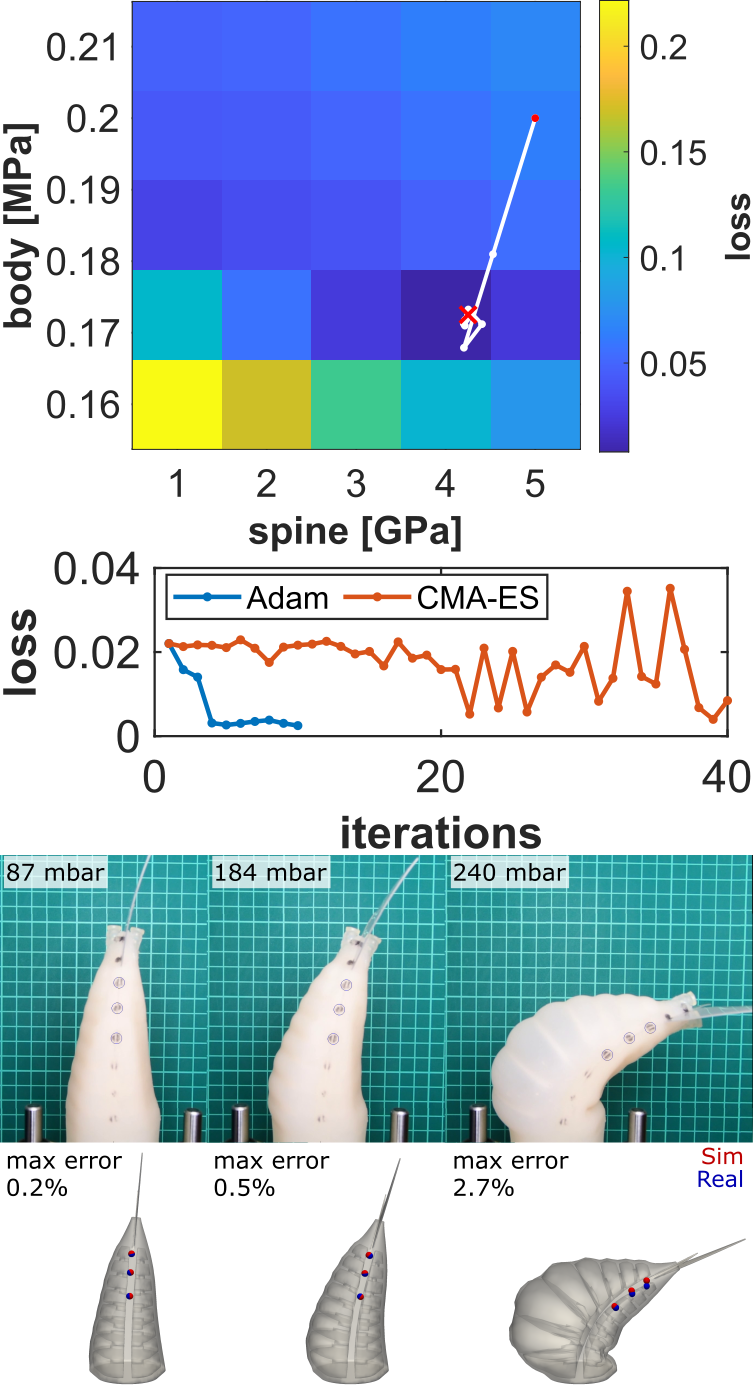
\includegraphics[width=0.85\columnwidth]{figures/grid_search_nemo_vertical_column.png}
    \caption{\textit{Top:} Exhaustive search of the Young's moduli pair for the spine and body. The moduli pair with the lowest Euclidean loss is located at the red $\times$. The red dot indicates the start of a gradient search and the white line shows the progress towards convergence. \textit{Middle:} Convergence comparison between a gradient-based (Adam) and gradient-free search (CMA-ES). \textit{Bottom:} Comparison of static deformation of the \emph{Nemo} fish for increasing pressure in experiment and simulation. Maximum displacement error increases with pressure, but remains within the measurement error (on the order of the diameter of markers). The grid in white under the real robot has \SI{10}{mm} spacing. The reported error is normalized to the fish tail length of \SI{10}{cm}.}
    \label{fig:system_id}
\end{figure}

\begin{figure}[t]
    \centering
    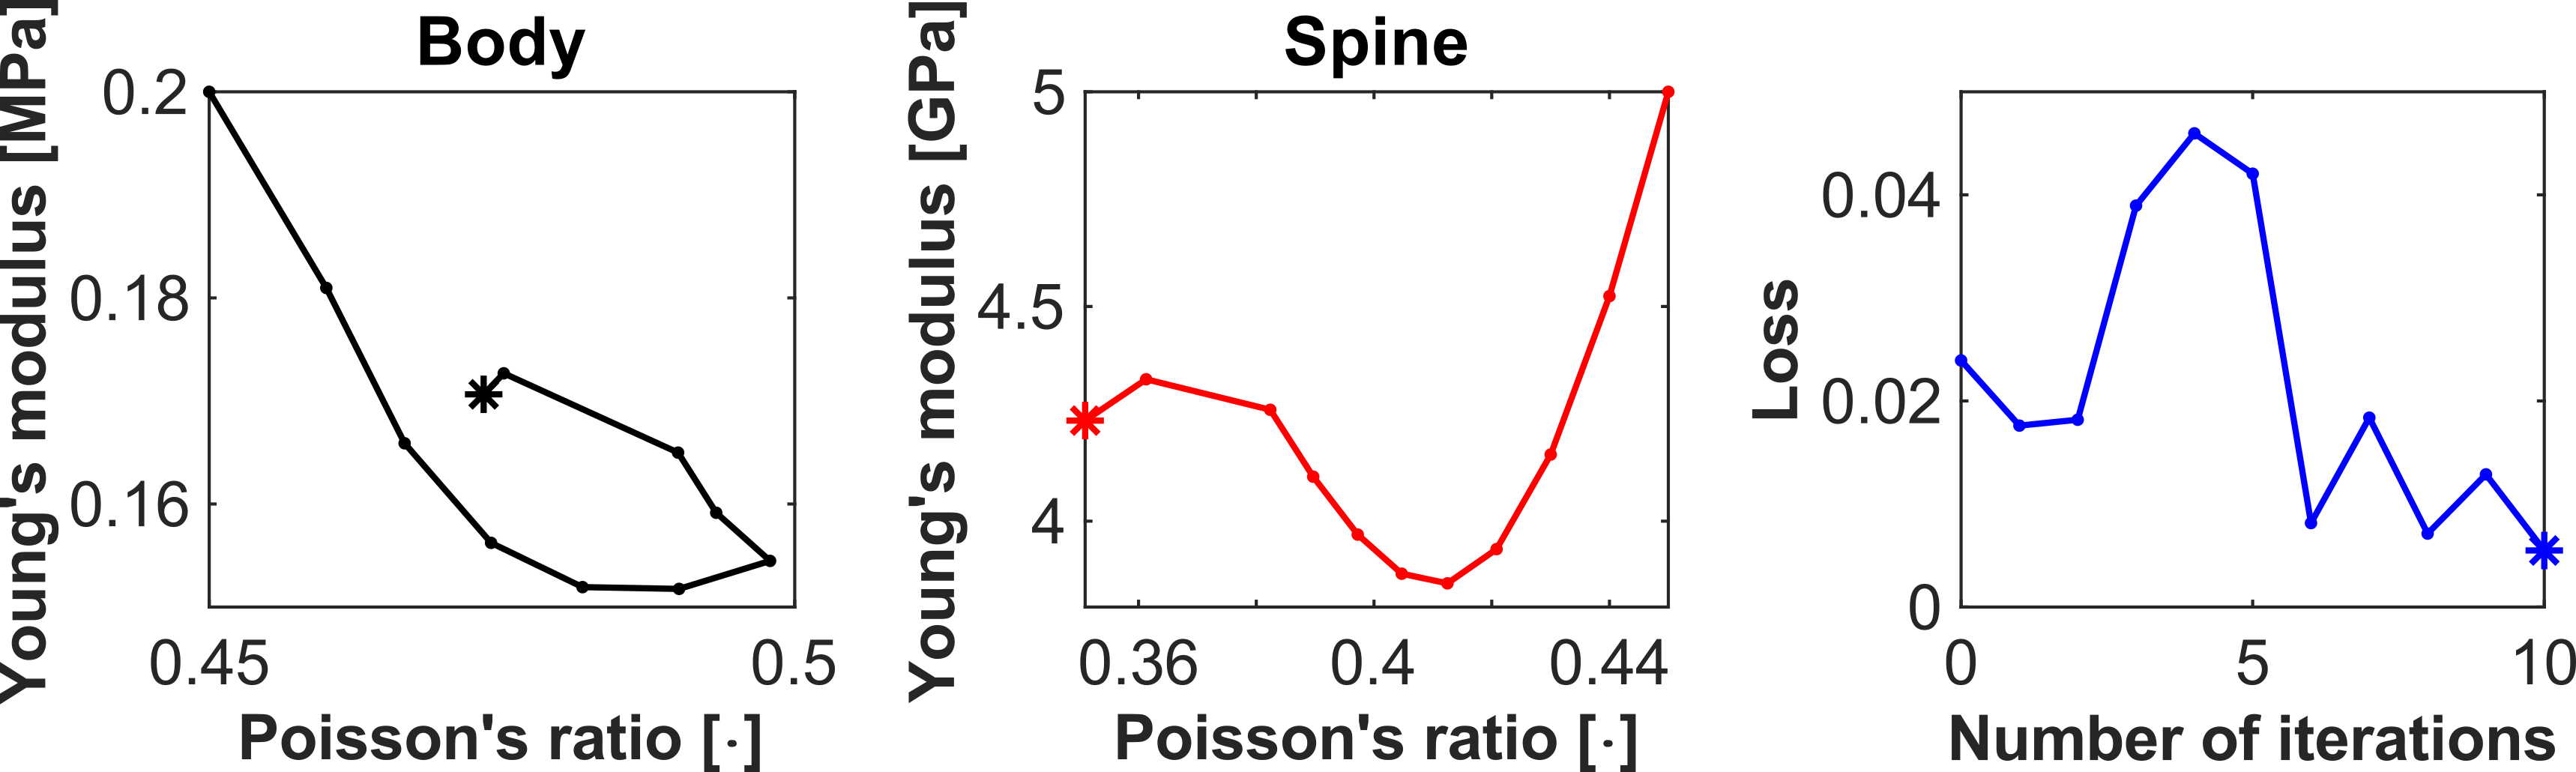
\includegraphics[width=0.99\columnwidth]{figures/param_search_figure_new.png}
    \caption{Learning four material parameters from deformation data take with the \textit{Nemo} fish prototype using a gradient-based approach that is run until convergence. The final values for Young's moduli and Poisson's ratios depicted as an asterisk agree with plausible material parameter values with lower loss.}
    \label{fig:4_param_search}
\end{figure}

For the \emph{Nemo} tail actuator described in \Cref{tab:fish}, we perform a grid search of the loss landscape centered around the ground truth datasheet values for the silicone and acetal materials of the body and spine. We report that if the exact geometry of the actuator is reproduced with high fidelity in the simulation, we converge to values within the range of typical measured values for the material Young's moduli (see \Cref{fig:system_id}). Further, we see that there is a unique minimum value that is within the acceptable range of measured moduli for both parameters. Note that we assume a priori that the Poisson ratio for silicone is $\nu\approx0.5$ or \textit{nearly} incompressible, a standard assumption for silicone, and the acetal sheet Poisson ratio is $\nu=0.37$ as reported by the manufacturer. Typical values for the Young's modulus of Dragon Skin 10 range from \SI{0.1}{MPa} to \SI{0.25}{MPa} and the value for Dragon Skin 20 was measured to be in the range of \SI{1.1}{MPa}~\cite{marechal2020toward} and typical values for the Young's modulus of acetal sheets range from \SI{2.5}{GPa} to \SI{5}{GPa}.\footnote{\url{https://dielectricmfg.com/knowledge-base/acetal/}}

In \Cref{fig:4_param_search}, we demonstrate that our method can be extended to higher dimensional parameter spaces such as a search over both Young's moduli and Poisson's ratios. Note that although we allow the Poisson ratio to vary in this identification experiment, the final value to which the body Poisson's ratio converges is still \textit{nearly} incompressible as expected for silicone.


\subsection{Gradient-based and Gradient-free Solver Methods}

We compare the runtime of the gradient-free method \emph{CMA-ES} against the runtime of the gradient-based method \emph{Adam} in \Cref{tab:gradient_methods}. The comparison shows that although \emph{CMA-ES}~\cite{igel2007covariance} is slightly faster in runtime per iteration, the use of the gradient-based method Adam~\cite{kingma2014adam} is significantly more effective for convergence. These comparative experiments shown in \Cref{fig:system_id} were carried out on a computer with an Intel Core i9-9900K @ 3.60GHz with 16 cores processor and 64.0 GB of memory.

\begin{table}[htb]
    \centering
    \caption{Comparison of Adam, CMA-ES, and Grid search. The forward simulation time is 318.9 seconds equivalent to grid search.}
    % \begin{tabular}{|p{10mm}|p{12mm}|p{12mm}|p{10mm}|p{17mm}|}
    \begin{tabular}{@{}lllll@{}}
        \toprule
        \thead[l]{Method} & \thead[l]{Total\\Iterations} & \thead[l]{Time Per\\ Iteration} & \thead[l]{Total Time} & \thead[l]{Loss After \\4 Iterations} \\
        \midrule
        \textbf{Adam} & \textbf{4} & 334.4 s & \textbf{~22 m} & \textbf{0.0027} \\
        CMA-ES & 40 & 321.0 s & ~214 m & 0.021  \\
        Grid search & 25 & \textbf{318.9 s} & 132.9 m & 0.023 \\
        \bottomrule
    \end{tabular}
    \label{tab:gradient_methods}
\end{table}

\subsection{Dynamic Experiments}

For dynamic experiments, we compare the results of our simulation output with the measured data of the furthest tracked dot on the tail. In Fig.~\ref{fig:results}, we report our findings for sim2real performance in both the standard fish (\emph{Nemo}) and two other data sets for a tail with different Young's moduli for the body (\emph{Bruce}) and a tail with a greater number of air chambers (\emph{Dory}). We demonstrate that if system identification is done correctly our simulation results can predict the performance of a novel actuator design to within millimeter precision or $3\%$ max normalized error using only a quasistatic data set for training without need for material testing. The \textit{Bruce} prototype required higher pressures to get similar displacements to \textit{Nemo} since the material is stiffer. The prototype \textit{Dory} required higher pressure as well to produce similar displacements due to a greater number of actuation chambers. For videos of the dynamic experiments and simulation, we ask readers to refer to our supplemental video.

\begin{figure}[t]
    \centering
    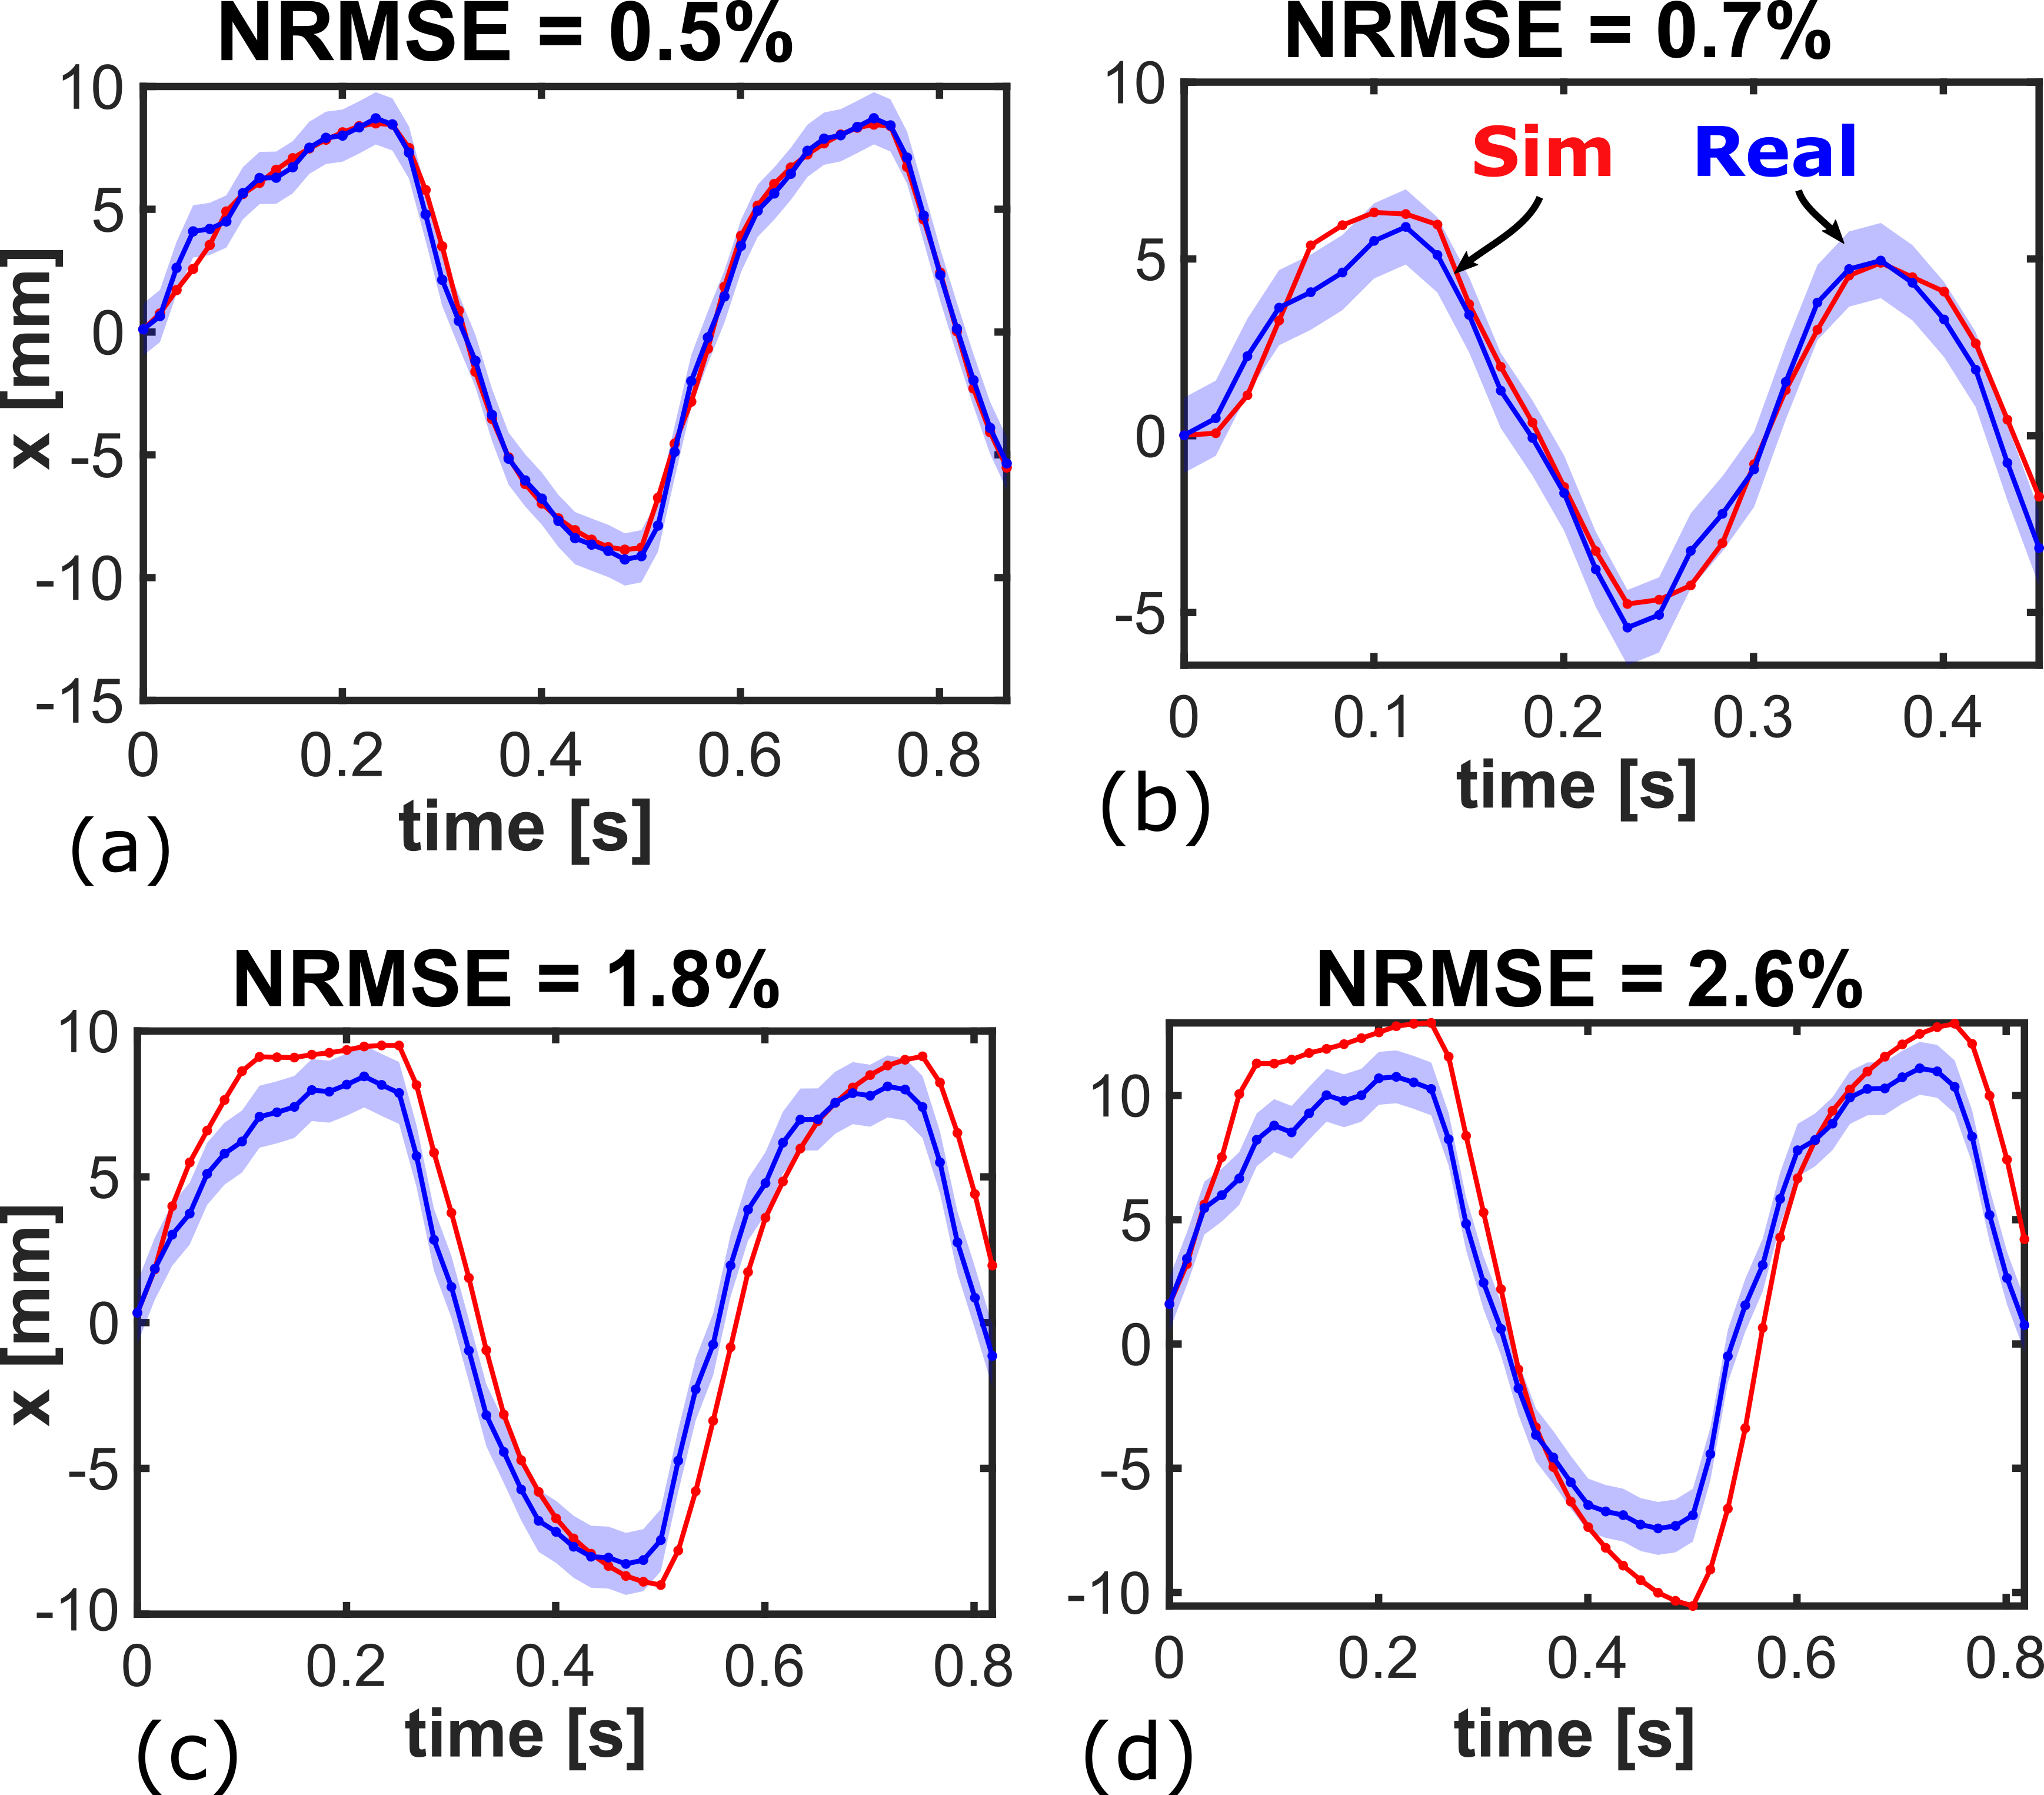
\includegraphics[width=0.85\columnwidth]{figures/dynamic_actuation_square.png}
    \caption{Simulation and measurement data for the \emph{Nemo} fish at (a) 200 mbar and 2 Hz, (b) 200 mbar and 4 Hz, (c) the \emph{Bruce} fish at 500 mbar and 2 Hz, and (d) the \emph{Dory} fish at 350 mbar and 2 Hz. The color bands indicate the variance from $N=5$ trials. For both actuation signals, we are capable of achieving sub-millimeter accuracy between experiment and simulation. The same method is used to identify the parameters of Bruce and Dory, exhibiting accuracy still within \SI{3}{mm}. We normalize the Root Mean Square Error (RMSE) to the fish tail length of \SI{10}{cm}. As expected, higher pressures result in larger deformations with greater error. The phase lag exhibited in \emph{Bruce} and \emph{Dory} may be due to actuator dynamics present during higher actuation pressures.}
    \label{fig:results}
    \vspace{-3pt}
\end{figure}

\subsection{Learned Hydrodynamics}
\label{sec:learned_hydrodynamics}
We compare our simple predictor of thrust force with the measurement data and the theoretical thrust from EBT, a classic, non-learning-based approximate analytical model from the literature, in~\Cref{fig:thrust_prediction}. Although the model is capable of generalizing to actuation signals at frequencies previously unobserved in the training for the \emph{Nemo} prototype, for the \emph{Bruce} prototype the discrepancy is large, nearly twice the measured force, likely because of the more limited training data.
In comparing to the thrust prediction from EBT, we see that the analytical thrust is strictly positive. The negative measured force is due to recoil of the measurement system. The advantage of our approach is the differentiability and flexibility of the neural network provided enough data is collected. We note that the network is capable of learning the measurement dynamics due to the compliance of the load cell and the damping of the water though these effects can be considered separately and corrected for if desired (see \Cref{sec:load_cell_measurement}). We conjecture that the asymmetry of the measured thrust may be due to imperfections in the fabrication process of the fish tails favoring one direction more strongly.

\begin{figure}[t]
    \centering
    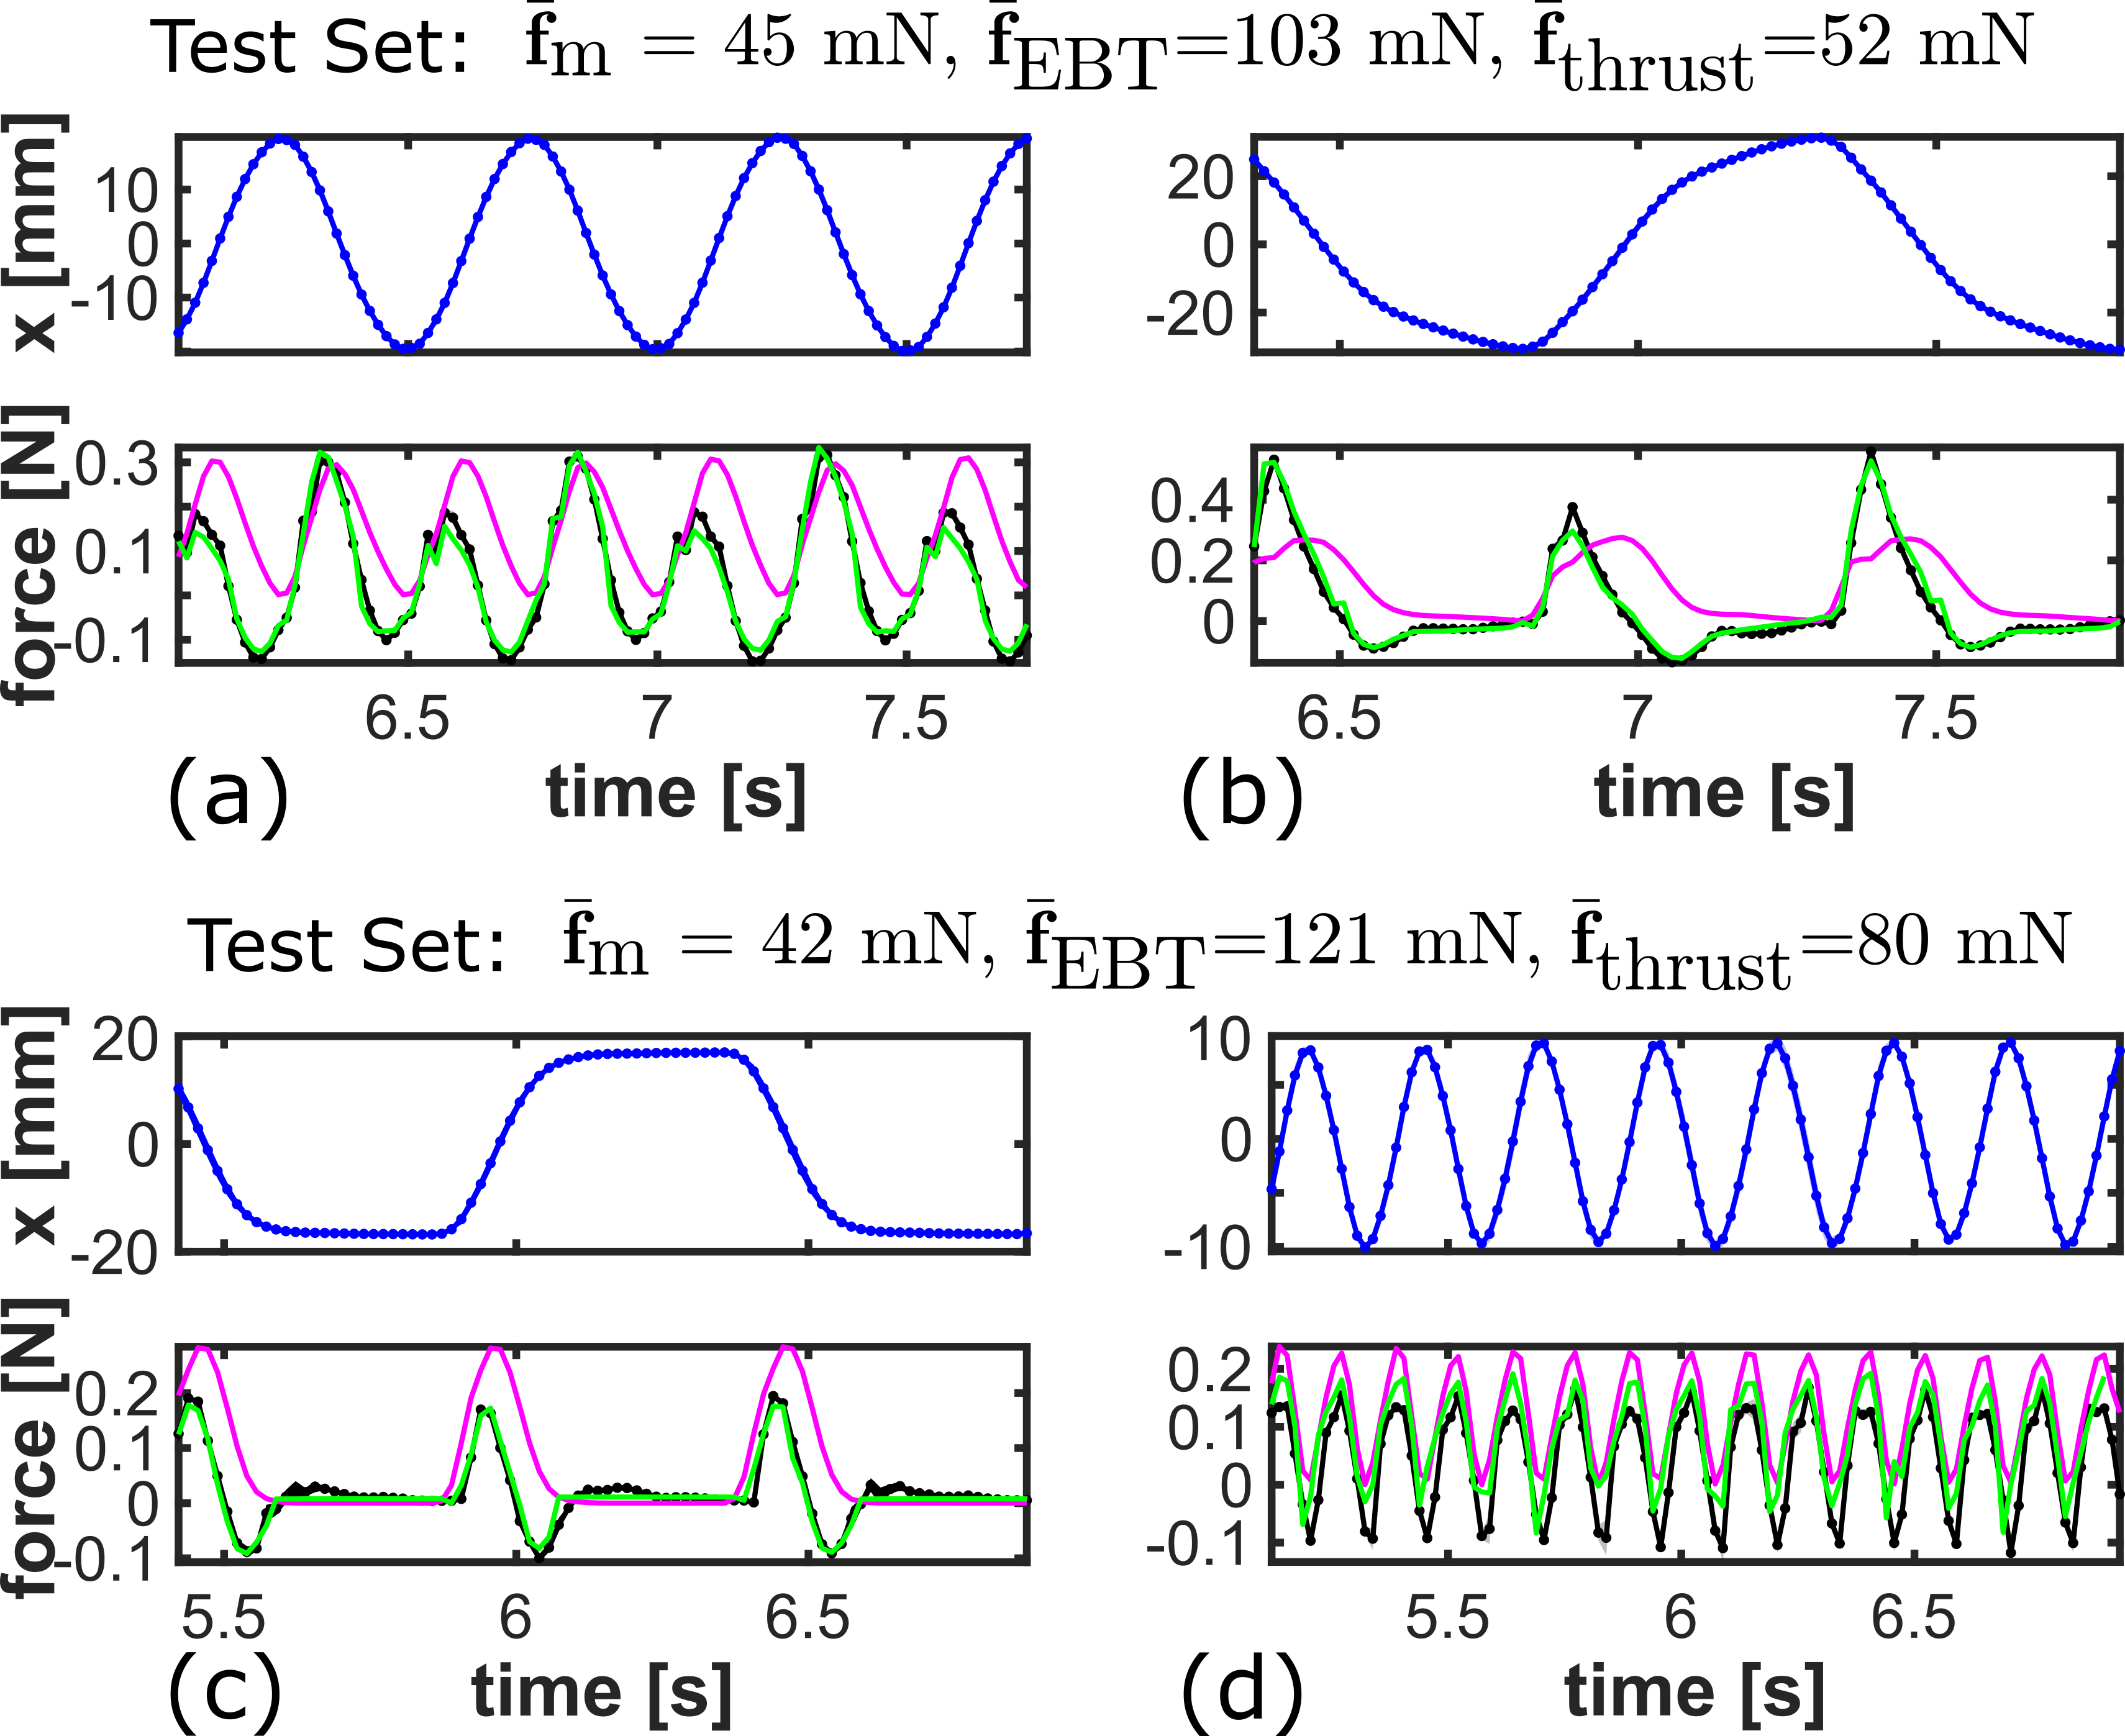
\includegraphics[width=1\columnwidth]{figures/hydrodynamics.png}
    \caption{Tail lateral displacement (blue) with thrust measurement and prediction. We compare the measured thrust force $\mathbf{f}_\textrm{m}$ (black), analytical thrust force from EBT $\mathbf{f}_\textrm{EBT}$ (magenta), and the neural network thrust prediction $\mathbf{f}_\textrm{thrust}$ (green). We show the thrust prediction for two training sets (a) and (c) and we report the time-averaged thrust for the two test cases (b) and (d). We note that EBT tends to over-predict the thrust measurement while our neural network thrust prediction accurately reproduces the frequency for a given actuation signal and matches amplitude more robustly than EBT.}
    \label{fig:thrust_prediction}
\end{figure}

\section{Conclusion}

Time series forecasting is an important business and research problem that has a broad impact in today's world. This paper proposes a novel Y-shaped architecture, specifically designed for the far horizon time series forecasting problem. The study shows the importance of direct connections from the multi-resolution encoder to the decoder and reconstruction loss for the task of time series forecasting. The Yformer couples the U-Net architecture from the image segmentation domain on a sparse transformer model and empirically demonstrates superior performance across multiple datasets for both univariate and multivariate settings. We believe that our work provides a base for future research in the direction of using efficient U-Net based skip connections and the use of reconstruction loss as an auxiliary loss within the time series forecasting community.

\subsubsection{Acknowledgements}: This work was supported by the Federal Ministry for Economic Affairs and Climate Action (BMWK), Germany, within the framework of the IIP-Ecosphere project (project number: 01MK20006D)
version https://git-lfs.github.com/spec/v1
oid sha256:acf082414844baa070da9f4ef2b0d8ae3ee7cf1d71ef93bfb27903fab9bf8ac2
size 6711


% \addtolength{\textheight}{-9cm}

\bibliographystyle{IEEEtran}
\bibliography{references}


\end{document}
